%
% matrixalgebra.tex
%
% (c) 2021 Prof Dr Andreas Müller, OST Ostschweizer Fachhochschule
%
\bgroup

\newtcbox{\myboxA}{blank,boxsep=0mm,
clip upper,minipage,
width=31.0mm,height=17.0mm,nobeforeafter,
borderline={0.0pt}{0.0pt}{white},
}
\definecolor{magenta}{rgb}{0.8,0.2,0.8}

\begin{frame}[t]
\frametitle{Matrix-Algebra}
\vspace{-10pt}
\[
\begin{pmatrix}
a_{11}&\dots &a_{1n}\\
\vdots&\ddots&\vdots\\
a_{m1}&\dots &a_{mn}
\end{pmatrix}
+
\begin{pmatrix}
b_{11}&\dots &b_{1n}\\
\vdots&\ddots&\vdots\\
b_{m1}&\dots &b_{mn}
\end{pmatrix}
=
\begin{pmatrix}
a_{11}+b_{11}&\dots &a_{1n}+b_{1n}\\
\vdots&\ddots&\vdots\\
a_{m1}+b_{m1}&\dots &a_{mn}+b_{mn}
\end{pmatrix}
\]
\[
\lambda
\begin{pmatrix}
a_{11}&\dots &a_{1n}\\
\vdots&\ddots&\vdots\\
a_{m1}&\dots &a_{mn}
\end{pmatrix}
=
\begin{pmatrix}
\lambda a_{11}&\dots &\lambda a_{1n}\\
\vdots&\ddots&\vdots\\
\lambda a_{m1}&\dots &\lambda a_{mn}
\end{pmatrix}
\]
\uncover<2->{%
\begin{center}
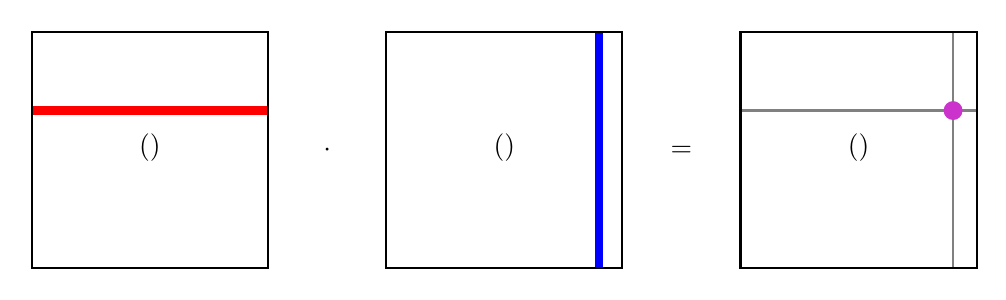
\begin{tikzpicture}[>=latex,thick]
\begin{scope}[xshift=-4.5cm]
\node at (1.5,1.53) {$\left(\myboxA{}\right)$};
\draw[color=red,line width=3pt] (0,2) -- (3,2);
\draw (0,0) rectangle (3,3);
\end{scope}
\node at (-0.75,1.5) {$\mathstrut\cdot\mathstrut$};
\begin{scope}[xshift=0cm]
\node at (1.5,1.53) {$\left(\myboxA{}\right)$};
\draw[color=blue,line width=3pt] (2.7,0) -- (2.7,3);
\draw (0,0) rectangle (3,3);
\end{scope}
\node at (3.75,1.5) {$\mathstrut=\mathstrut$};
\begin{scope}[xshift=4.5cm]
\node at (1.5,1.53) {$\left(\myboxA{}\right)$};
\draw[color=gray,line width=1pt] (2.7,0) -- (2.7,3);
\draw[color=gray,line width=1pt] (0,2) -- (3,2);
\fill[color=magenta] (2.7,2) circle[radius=0.12];
\draw (0,0) rectangle (3,3);
\end{scope}
\end{tikzpicture}
\end{center}}
\end{frame}

\egroup
